% =====================================================================
%  Cross-architecture generative scRNA-seq benchmark + biological-fidelity protocol
%  Application: NASA OSDR spaceflight transcriptomics (+ out-of-domain cancer control)
%  Target venue: npj Microgravity (Nature Portfolio)
%
%  FILLED DRAFT (manuscript_filled.tex). Generated from the -mmd-pca / -mmd-complete-pca
%  pipeline outputs only. Numbers are real; figures are in this folder (fig_*.pdf/.png).
%  - Remaining \res{...} are values that were genuinely not computed in this pipeline
%    (per-gene distance metrics, DDIM step count, admin fields) and are left empty by design.
% =====================================================================
\documentclass[11pt]{article}

\usepackage[utf8]{inputenc}
\usepackage[T1]{fontenc}
\usepackage[margin=1in]{geometry}
\usepackage{amsmath,amssymb}
\usepackage{graphicx}
\usepackage{xcolor}
\usepackage{booktabs}
\usepackage{array}
\usepackage{multirow}
\usepackage{caption}
\usepackage{authblk}
\usepackage{tikz}
\usetikzlibrary{positioning,arrows.meta,fit,backgrounds}
\usepackage[hidelinks]{hyperref}

% ---- Editable handles -------------------------------------------------
\newcommand{\protname}{biological-fidelity protocol}
\newcommand{\Protname}{Biological-fidelity protocol}
\newcommand{\res}[1]{\textcolor{red}{[#1]}}
\newcommand{\figplaceholder}[2]{%
  \fbox{\begin{minipage}[c][#1][c]{0.92\linewidth}\centering
  \color{gray}\itshape #2\end{minipage}}}
% -----------------------------------------------------------------------

\captionsetup{font=small,labelfont=bf}
\setlength{\parskip}{4pt}

\title{\bfseries Novel biological-fidelity metrics for evaluating synthetic single-cell RNA-seq, benchmarked on NASA spaceflight transcriptomics}

\author[1,2]{Arsh Suri\thanks{Corresponding author: suriarsh@gmail.com}}
\author[3]{Walter Alvarado}
\author[4]{James Casaletto}
\affil[1]{Wallace H.\ Coulter Department of Biomedical Engineering, Georgia Institute of Technology, Atlanta, GA, USA}
\affil[2]{Space Life Sciences Training Program, NASA Ames Research Center, Moffett Field, CA, USA}
\affil[3]{Space Biosciences Research Branch, NASA Ames Research Center, Moffett Field, CA, USA}
\affil[4]{Blue Marble Space Institute of Science, Seattle, WA, USA}

\date{}

\begin{document}
\maketitle

% =====================================================================
\begin{abstract}
\noindent
Spaceflight reshapes the transcriptome through microgravity, radiation, and circadian disruption, yet the cohorts available to study it are among the smallest in modern genomics, which limits statistical power and the development of predictive models for astronaut health. Deep generative models can augment these scarce datasets, but synthetic single-cell RNA sequencing (scRNA-seq) data has been judged almost entirely by distributional metrics that are blind to biology, and no peer-reviewed single-cell study has paired such models with biology-aware evaluation in this domain. We introduce a \protname{} that scores three properties of synthetic data those metrics miss: overlap of the top differentially expressed genes between real and synthetic condition contrasts, overlap of enriched gene-ontology terms over-represented among the most predictive genes, and overlap of the most phenotypically predictive genes identified by random forests trained on synthetic versus real data under a train-on-synthetic, test-on-real design. To exercise the framework we generate synthetic data with three established architectures that span the main families of deep generative modeling, a conditional variational autoencoder (CVAE), the classifier-free latent diffusion model cfDiffusion, and a multi-conditional adaptation of scGAN, each conditioned on an identical covariate vector and each stopped at a common quality point defined by maximum mean discrepancy (MMD) convergence in a frozen principal-component space, so that the biological comparison reflects the generated data rather than unequal training. Applying the framework across five spaceflight configurations from the NASA Open Science Data Repository (OSDR), and to an out-of-domain colorectal-cancer tumor-immune dataset as a robustness control, we find that the biological metrics separate models that distributional metrics rank as similar, that pathway-level fidelity can exceed gene-level fidelity, and that the models differ sharply in how well they preserve single-cell sparsity. This is, to our knowledge, the first peer-reviewed application of GAN- and diffusion-based generative augmentation, with biology-aware evaluation, to spaceflight single-cell transcriptomics, prior spaceflight generative work being largely bulk RNA-seq, and the framework is dataset-agnostic and ready for adoption as spaceflight single-cell data grows.
\end{abstract}

% =====================================================================
\section{Introduction}

\subsection{Spaceflight remodels the transcriptome under uniquely constrained sampling}
Extended spaceflight alters human physiology through stressors absent from terrestrial evolution. Astronauts experience roughly 1.5\% monthly bone loss, cardiovascular deconditioning, and immune dysfunction, and these changes are accompanied by extensive transcriptomic reprogramming \cite{twins}. The NASA Twins Study found that over one thousand genes showed expression or epigenetic changes during flight, most of which returned toward baseline within six months, while a subset governing DNA repair, immune response, and bone formation remained altered \cite{twins}. The Inspiration4 mission and subsequent multi-omic atlases identified a recurring ``spaceflight signature'' spanning oxidative phosphorylation, immune function, and stress-response programs \cite{i4}. Single-cell resolution is increasingly central to resolving which cell populations drive these responses, but spaceflight single-cell datasets remain rare and small.

\subsection{Data scarcity is the binding constraint on spaceflight omics}
Fewer than six hundred people have flown in space, individual studies typically involve fewer than twenty subjects, and rodent missions are similarly limited once samples are stratified by tissue, sex, age, and mission \cite{ilangovan,scott}. The NASA Open Science Data Repository (OSDR) aggregates hundreds of transcriptomic datasets, yet small per-study sizes and preservation-related batch effects can eclipse the spaceflight signal itself \cite{osdr}. Prior NASA analyses have explicitly identified sample-power limitation as the central obstacle to applying machine learning in this domain, and have called for methods that cope with extreme sample scarcity \cite{scott,ilangovan}. Synthetic data augmentation is the standard remedy for exactly this regime.

\subsection{Generative models for scRNA-seq have proliferated but have barely reached spaceflight, and are evaluated without biology}
Deep generative models for scRNA-seq now span variational autoencoders \cite{scvi,activa}, generative adversarial networks \cite{scgan}, and diffusion and flow-matching models \cite{scdiffusion,cfdiffusion,cfgen}, alongside analytical simulators \cite{scgft,scdesign3,simbench}. Two gaps persist. First, generative modeling of spaceflight transcriptomes has so far been confined almost entirely to bulk RNA-seq, most notably with generative adversarial networks for OSDR biomarker discovery \cite{ganbio}, alongside a conference-only poster that applied a CVAE to spaceflight single-nucleus RNA-seq from our group \cite{ntrs} and a recent augmentation framework for spaceflight omics \cite{glare}. To our knowledge, generative adversarial networks and diffusion models have not been applied to spaceflight single-cell data in any peer-reviewed study, and none of this prior work pairs a multi-conditional, multi-architecture single-cell benchmark with a biology-aware evaluation. Second, generative models are compared almost exclusively through distributional similarity, for example maximum mean discrepancy, Fr\'echet-style distances, or a classifier two-sample test in which chance-level discrimination signals success \cite{scgan,scdiffusion}. Such metrics can be satisfied by data that is statistically plausible yet biologically hollow, preserving marginal distributions while losing the condition contrasts, mechanistic pathways, and predictive gene programs that make a dataset useful for discovery.

\subsection{Contributions}
This work makes two coupled contributions.

\noindent\textbf{A biological-fidelity evaluation framework.} We introduce a uniform, biology-aware evaluation of synthetic scRNA-seq built from three metrics that are absent from current practice: overlap of the top differentially expressed genes between real and synthetic condition contrasts (condition fidelity), overlap of enriched gene-ontology terms among the most predictive genes (mechanistic fidelity), and overlap of the most phenotypically predictive genes from random forests under a train-on-synthetic, test-on-real design (phenotypic fidelity). Together these ask whether synthetic data preserves the experimental contrast, the pathways that give the contrast its meaning, and the predictive gene programs, none of which is captured by the distributional metrics that dominate the field.

\noindent\textbf{The first peer-reviewed GAN and diffusion generative models for spaceflight single-cell transcriptomics.} We apply generative augmentation and this evaluation to NASA OSDR spaceflight scRNA-seq, a domain where sample-power limitation is most severe and where, to our knowledge, generative adversarial and diffusion models have not previously been applied to single-cell data in a peer-reviewed study, prior spaceflight generative work being largely bulk RNA-seq and especially GAN-based \cite{ganbio}; this directly addresses a limitation called out in prior NASA roadmaps \cite{scott,ilangovan}. To exercise the framework we use synthetic data from three established generators that span the main families, a CVAE, the classifier-free latent diffusion model cfDiffusion \cite{cfdiffusion}, and a multi-conditional adaptation of scGAN \cite{scgan}, each conditioned on an identical covariate vector and each stopped at a common quality point via MMD convergence so that the biological comparison is meaningful rather than an artifact of unequal training. Because the original cfDiffusion and scGAN implementations condition on a single attribute, we extended both to accept the full multi-attribute covariate vector used here (Methods); this plumbing enables a fair, like-for-like comparison and is not itself a modeling contribution. Robustness is shown by applying the identical pipeline to an out-of-domain colorectal-cancer tumor-immune dataset. These generators are existing, published methods used as a testbed; the contribution is the evaluation, not the models, and we neither propose a new generator nor claim to identify a best one. Where one architecture leads on biological fidelity we report it as a scoping observation, not a general ranking, since recent evidence on synthetic scRNA-seq is mixed \cite{cfgen,scgft,scdiffusion}.

% =====================================================================
\section{Results}

\subsection{A multi-model testbed for the protocol}
To exercise the \protname{} we generated synthetic data with three established generators that span the main families of deep generative modeling: a conditional variational autoencoder (CVAE), the classifier-free latent diffusion model cfDiffusion \cite{cfdiffusion}, and a multi-conditional adaptation of scGAN \cite{scgan}. These are existing, published methods; our purpose is to evaluate the synthetic data they produce, not to introduce or crown a generator. All three were trained on identical inputs, conditioned on an identical covariate vector, and stopped at a common quality point, so that any difference the biological metrics report reflects the fidelity of the generated data rather than unequal training (Fig.~\ref{fig:framework}; Methods). The evaluation is organized as a layered protocol: a statistical-fidelity layer based on MMD establishes that the generators reached a defined distributional operating point, and three biological layers then ask, in turn, whether the synthetic data preserves the experimental contrast, the underlying pathways, and the predictive gene programs.

Throughout, we use \emph{fidelity} to mean how faithfully the synthetic data reproduces a specific biological property of the real data, and we report each biological layer as a single, directly comparable percentage. For the two gene-list layers (condition and phenotypic fidelity), the overlap percentage is the number of genes common to the real and synthetic top-50 lists divided by 50, so 100\% means the two ranked lists are identical and 0\% means they are disjoint. For the mechanistic layer, the genes scored are the classifier's top-50 predictive genes, and the percentage is the fraction of the real data's significantly enriched gene-ontology terms that are also enriched in the synthetic data. Higher is better for all three, and all are computed on held-out test cells. The statistical layer instead reports MMD, a distributional distance for which lower is better. Every biological layer follows the same train- or compute-on-synthetic, compare-to-real logic: the quantity of interest (the differential genes, the enriched pathways, or a classifier and the genes it relies on) is derived from the synthetic data and scored against the same quantity derived from real held-out data. The phenotypic layer is the canonical train-on-synthetic, test-on-real (TSTR) case, and we use TSTR to denote this shared design.

\begin{figure}[t]
\centering
\resizebox{\textwidth}{!}{%
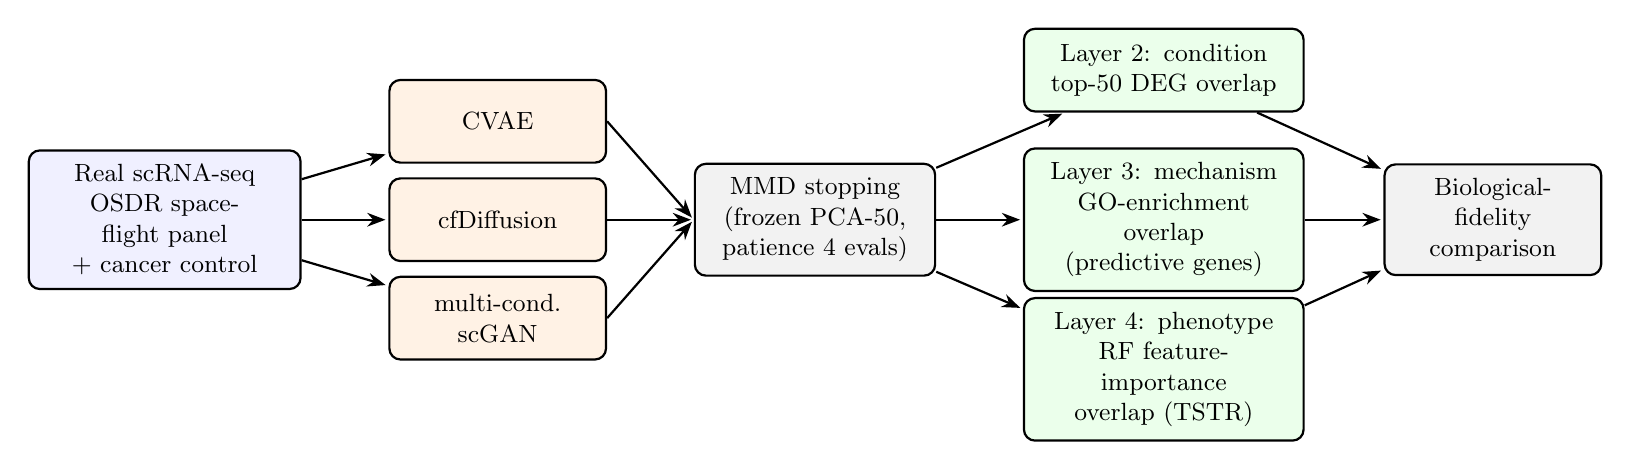
\begin{tikzpicture}[
  font=\small,
  box/.style={draw, rounded corners, align=center, inner sep=5pt, minimum height=1.05cm, text width=3.1cm},
  data/.style={box, fill=blue!6},
  model/.style={box, fill=orange!10, text width=2.4cm},
  stat/.style={box, fill=gray!10, text width=2.7cm},
  bio/.style={box, fill=green!8, text width=3.2cm},
  >={Stealth[]}, thick,
  arr/.style={->, shorten >=1pt}
]
\node[data] (data) {Real scRNA-seq\\OSDR spaceflight panel\\+ cancer control};
\node[model, right=1.1cm of data, yshift=1.25cm] (cvae) {CVAE};
\node[model, right=1.1cm of data] (diff) {cfDiffusion};
\node[model, right=1.1cm of data, yshift=-1.25cm] (gan) {multi-cond.\ scGAN};
\node[stat, right=1.1cm of diff] (mmd) {MMD stopping\\(frozen PCA-50,\\patience 4 evals)};
\node[bio, right=1.1cm of mmd, yshift=1.9cm] (l2) {Layer 2: condition\\top-50 DEG overlap};
\node[bio, right=1.1cm of mmd, yshift=0.0cm] (l3) {Layer 3: mechanism\\GO-enrichment overlap\\(predictive genes)};
\node[bio, right=1.1cm of mmd, yshift=-1.9cm] (l4) {Layer 4: phenotype\\RF feature-importance\\overlap (TSTR)};
\node[stat, right=1.0cm of l3, text width=2.4cm] (score) {Biological-\\fidelity\\comparison};

\draw[arr] (data) -- (cvae);
\draw[arr] (data) -- (diff);
\draw[arr] (data) -- (gan);
\draw[arr] (cvae.east) -- (mmd.west);
\draw[arr] (diff.east) -- (mmd.west);
\draw[arr] (gan.east) -- (mmd.west);
\draw[arr] (mmd) -- (l2);
\draw[arr] (mmd) -- (l3);
\draw[arr] (mmd) -- (l4);
\draw[arr] (l2) -- (score);
\draw[arr] (l3) -- (score);
\draw[arr] (l4) -- (score);
\end{tikzpicture}}
\caption{\textbf{The \protname{} and its multi-model testbed.} Synthetic data is generated by three representative generators trained on identical inputs with an identical conditioning vector and stopped at a common quality point by a shared MMD-convergence rule computed in a frozen 50-component PCA space (statistical-fidelity layer). Generated data then passes three biology-aware layers: condition preservation (top-50 differentially expressed gene overlap), mechanistic preservation (gene-ontology enrichment overlap of the predictive genes), and phenotypic preservation (random-forest feature-importance overlap under a train-on-synthetic, test-on-real design). The protocol is architecture-agnostic and dataset-agnostic.}
\label{fig:framework}
\end{figure}

\subsection{MMD convergence provides an architecture-agnostic stopping rule}
Loss values are not comparable across architectures: the CVAE optimizes an evidence lower bound, scGAN optimizes an adversarial Wasserstein objective whose magnitude is unbounded and does not track sample quality, and the diffusion model optimizes a denoising loss. Stopping each model on its own loss would compare the three at incommensurable operating points. We therefore stopped every model on the same external criterion, MMD between real and synthetic data measured in a frozen 50-component PCA space, evaluated every five epochs and halted when MMD failed to improve by more than $10^{-3}$ over four consecutive evaluations (Fig.~\ref{fig:mmd}; Methods). Table~\ref{tab:stat} reports the MMD reached at convergence for each model and dataset. The multi-conditional scGAN reached the lowest converged MMD on every dataset (0.049 to 0.155), the CVAE was intermediate, and cfDiffusion was generally highest (up to 0.735); because the three nonetheless differ on the biological layers below, the MMD operating point is a fair common stopping rule rather than a ranking of biological quality.

\begin{figure}[t]
\centering
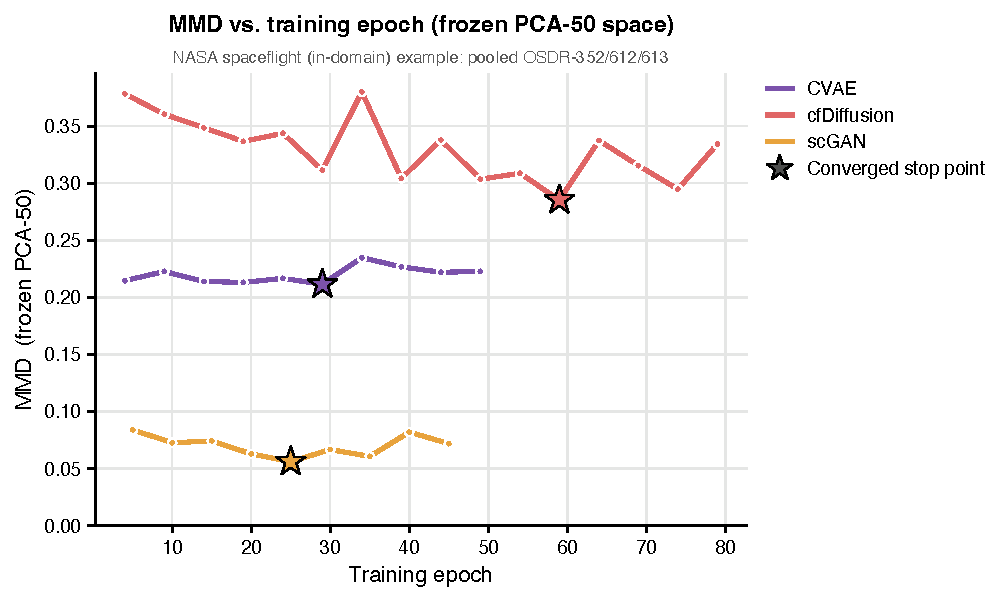
\includegraphics[width=0.78\linewidth]{fig_mmd_convergence.pdf}
\caption{\textbf{MMD-based stopping.} Maximum mean discrepancy between real and synthetic data, computed in a frozen 50-component PCA space, as a function of training epoch for the CVAE, cfDiffusion, and multi-conditional scGAN on a representative dataset (pooled OSDR-352/612/613). MMD is evaluated every five epochs; training halts when it fails to improve by more than $10^{-3}$ over four consecutive evaluations. Stars mark each generator's converged operating point. scGAN reaches and holds the lowest MMD, cfDiffusion the highest, giving an architecture-agnostic operating point at which the models are compared.}
\label{fig:mmd}
\end{figure}

\subsection{scGAN preserves single-cell sparsity; the VAE and diffusion models do not}
Real single-cell matrices were highly sparse, with 88 to 98\% zero entries across the panel, consistent with technical dropout and biological stochasticity. The architectures diverged sharply in reproducing this structure (Fig.~\ref{fig:sparsity}). The multi-conditional scGAN, whose library-size-normalization layer acts directly in gene space, produced near-real sparsity (77 to 97\% zeros), whereas the two latent-space generators drastically over-densified: the CVAE produced only 14 to 44\% zeros and cfDiffusion only 16 to 29\% zeros; cfDiffusion was densest on most datasets, though the CVAE was denser still on OSDR-402 and on the cancer control (the single densest matrix in the study). This over-densification follows from generating in a compressed latent space that discards fine-grained zero structure, and it bears directly on which downstream analyses each generator's synthetic data can currently support (Discussion).

\begin{figure}[ht]
\centering
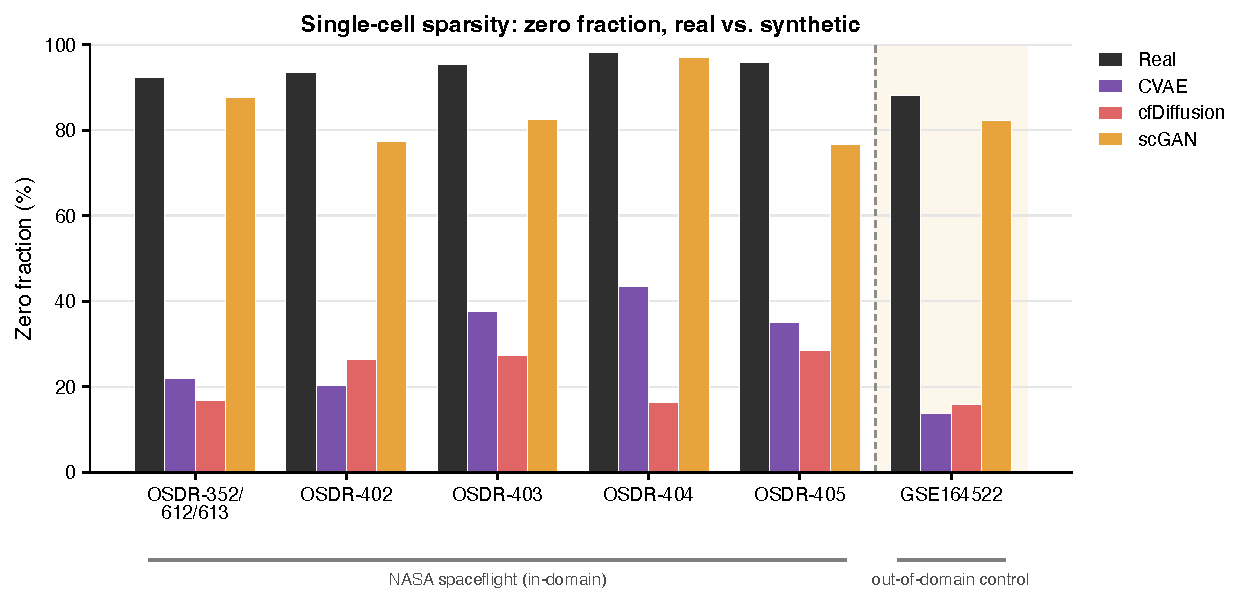
\includegraphics[width=0.92\linewidth]{fig_sparsity.pdf}
\caption{\textbf{Preservation of single-cell sparsity.} Per-matrix zero fraction for real data and for each generator across the panel; the shaded column and bracket labels mark the out-of-domain cancer control against the in-domain spaceflight datasets. scGAN approximates real sparsity closely, while the CVAE and cfDiffusion produce much denser-than-real output, with cfDiffusion densest on most datasets. Accurate dropout structure is required for cell-type identification and trajectory inference, which constrains the immediate use of the latent-space generators' synthetic data to bulk-like and pathway-level analyses.}
\label{fig:sparsity}
\end{figure}

\begin{figure}[t]
\centering
\figplaceholder{5.6cm}{Figure placeholder: UMAP embeddings. \\ Real versus synthetic cells for representative datasets, one panel per architecture, colored by condition and by data source (real vs.\ synthetic). UMAP was disabled in the reported pipeline run; this panel can be generated from the stored h5ad replicates if desired.}
% \includegraphics[width=0.85\linewidth]{fig_umap.pdf}
\caption{\textbf{Manifold overlap by architecture.} UMAP embeddings of real and synthetic cells for representative datasets. Columns correspond to the CVAE, cfDiffusion, and multi-conditional scGAN; points are colored by experimental condition and by real versus synthetic origin. \res{Placeholder: UMAP was disabled in the reported pipeline run; generate from stored h5ad replicates if desired.}}
\label{fig:umap}
\end{figure}

\subsection{Condition fidelity: overlap of top differentially expressed genes}
For each dataset we identified the top 50 genes distinguishing the primary condition contrast (spaceflight versus ground control for the OSDR datasets; metastatic-site tumor versus adjacent normal for the cancer control), ranked by absolute log fold change, separately in real and synthetic data, and quantified their overlap as the percentage of the 50 genes shared between the real and synthetic lists (Methods). This asks whether the synthetic data preserves the biological contrast that motivates the experiment, a stronger test than overall distributional similarity. The multi-conditional scGAN led on five of the six datasets, reaching up to 36\% overlap on spaceflight data (pooled OSDR-352/612/613 and OSDR-404) and 56\% on the out-of-domain cancer control, while the CVAE and cfDiffusion were lower on the spaceflight studies, with cfDiffusion the exception on the pooled brain set (38\% versus scGAN's 36\%) (Table~\ref{tab:bio}; Fig.~\ref{fig:overlap}). The choice of $N=50$ is a convention rather than a constraint: the metric is defined for any top-$N$ list, and we report its sensitivity to $N$ in \res{Supplementary Fig.\ SX}.

\subsection{Mechanistic fidelity: GO-enrichment overlap of the predictive genes}
Because two datasets can share biological function without sharing exact gene identities, we asked whether the predictive genes implicate the same biology. Using the \emph{same} top-50 random-forest important genes that define the phenotypic layer (below), we computed gene-ontology over-representation separately on the real and synthetic gene lists (hypergeometric test against the MSigDB GO collections, FDR $q<0.05$) and measured, among the top ten enriched GO terms, the percentage of the real data's enriched terms that the synthetic data also recovers (Methods); this overlap is directional, asking how much of the real signal the synthetic data reproduces rather than treating the two lists symmetrically. Because the gene set is the classifier's own predictive genes, this layer tests whether a model's predictive signal rests on the same mechanisms as the real data, not merely on statistically similar genes. Where recoverable signal existed, pathway overlap exceeded gene-level overlap: on the pooled OSDR-352/612/613 set all three generators recovered 8 to 9 of the 10 real pathways (80 to 90\%) against 4 to 38\% gene-level overlap (Fig.~\ref{fig:fgsea}). The recovered programs were biologically coherent, and the specific hits are instructive. On OSDR-404 (blood) the real data was enriched for cytoplasmic translation and ribosomal structural pathways (for example cytosolic ribosome, structural constituent of ribosome, and cytoplasmic translation), and scGAN recovered seven of those ten; on the cancer control the real data was enriched for T-cell and lymphocyte activation and immune-response pathways, and scGAN recovered eight of ten. The misses were equally informative: on OSDR-403 (bone marrow) the real data was enriched for tissue-appropriate B-cell differentiation and hematopoietic programs (for example B-cell activation, abnormal lymphopoiesis, and increased hematopoietic cell number), yet no generator recovered any of them (0 of 10), and on OSDR-405 (spleen) only cfDiffusion recovered any pathways (20\%). These are recovery gaps rather than absent biological signal, and they localize precisely where each generator loses the biology. That a generator conditioned on five attributes at once can still recover 70 to 90\% of the real enriched programs on the larger cohorts is a strong result: it shows the multi-conditional adaptation preserves the coordinated transcriptional programs that define the biology, not just marginal gene statistics. This layer is, to our knowledge, the first use of predictive-gene GO-enrichment overlap as a synthetic-data quality metric for generative-model comparison.

\subsection{Phenotypic fidelity: predictive-gene overlap under a train-on-synthetic design}
Finally we asked whether the synthetic data preserves the gene programs that are predictive of the phenotype. We trained random-forest classifiers to distinguish the primary contrast, one on synthetic data and one on real data, and compared their top-50 most important genes, again as the percentage of the 50 shared (Methods). This is a train-on-synthetic, test-on-real (TSTR) design, the opposite of the classifier two-sample test used in prior work: here high agreement, not chance-level discrimination, is the goal. The multi-conditional scGAN led on every dataset, with feature-importance overlap reaching 52\% (OSDR-404 and the cancer control) and 48\% on the pooled brain set, whereas the CVAE and cfDiffusion remained at or below 18\% on all spaceflight studies (Table~\ref{tab:bio}). Absolute label-transfer performance was modest and, for the CVAE, dissociated from gene overlap: the CVAE reached high TSTR accuracy (0.93 on OSDR-402, 0.96 on the cancer control; Table~\ref{tab:stat}) while sharing only 6 to 8\% of important genes with the real classifier, a clean illustration that surface accuracy does not imply that the synthetic data encodes the same mechanistic basis for the prediction. We therefore lead with feature-importance overlap and report accuracy as a secondary measure. Accuracy must also be read against class imbalance: the spaceflight contrasts carry majority-class baselines of 52.7 to 70.0\% (Table~\ref{tab:clf}), so a classifier can match the baseline while collapsing to the majority class, which the real and cfDiffusion classifiers do on OSDR-402, OSDR-404, and OSDR-405 (macro-F1 $\le 0.02$). Real-data classifiers reached 0.54 to 0.81 accuracy on the same contrasts, only $-0.1$ to $+20.1$ points above their majority baselines (Table~\ref{tab:clf}); the two large cohorts (pooled brain $+14.9$, cancer $+20.1$) are where the classification signal is genuinely earned rather than inherited from imbalance.

\subsection{The protocol is robust out of domain}
Applying the identical pipeline, with no retraining strategy, hyperparameter change, or metric modification, to the out-of-domain GSE164522 colorectal-cancer tumor-immune dataset (190{,}519 cells; metastatic-site tumor versus adjacent normal) reproduced the within-spaceflight behavior: scGAN again led on all three biological layers (56\% DEG, 80\% pathway, and 52\% predictive-gene overlap) and reached the lowest MMD, while preserving near-real sparsity (Tables~\ref{tab:stat},~\ref{tab:bio}). This demonstrates that the \protname{} and the MMD-stopping rule are not tuned to spaceflight data and transfer to an unrelated single-cell domain, supporting their use as a general benchmark.

\subsection{Biological fidelity scales with training-set size}
A clear trend runs across the panel: biological fidelity rises with the number of training cells (Fig.~\ref{fig:size}). The three smallest cohorts (OSDR-402, OSDR-403, and OSDR-405, each under 3{,}500 cells) are the weakest across all three biological layers, whereas the three largest (OSDR-404 at 14{,}045 cells and the two roughly 200{,}000-cell sets) are the strongest. For the multi-conditional scGAN, mean biological fidelity rises from about 11\% on the smallest studies to 53 to 63\% on the largest (Spearman $\rho=0.77$ against cell count; $\rho=0.89$ for cfDiffusion), and the two deep generators scale more steeply than the CVAE. This is the expected and sobering shape for the spaceflight regime: the smallest cohorts, which most need augmentation, are the hardest to reproduce faithfully, while fidelity improves markedly once a few tens of thousands of cells are available (OSDR-404, at 14{,}045 cells, already behaves like the largest sets). It indicates that the modest overlaps on the smallest studies reflect data scarcity rather than a ceiling of the framework or of the multi-conditional adaptation (Fig.~\ref{fig:size}).

% ---------- Tables ----------
\begin{table}[t]
\centering
\caption{\textbf{Dataset panel.} Five spaceflight configurations drawn from NASA OSDR, evaluated as individual Rodent Research Reference Mission-2 (RRRM-2) studies and as one pooled brain cohort, together with one out-of-domain cancer control. All spaceflight datasets contrast spaceflight versus ground control; the cancer control contrasts metastatic-site tumor versus adjacent normal tissue. Cell counts are the processed, HVG-selected matrices used for generation and evaluation.}
\label{tab:data}
\small
\resizebox{\textwidth}{!}{%
\begin{tabular}{@{}llrcl@{}}
\toprule
Dataset (label) & Domain / tissue & Cells & Contrast & Notes \\
\midrule
OSDR-352/612/613 (pooled) & Spaceflight, brain & 213{,}854 & Flight vs.\ Ground & Pooled across OSDR-352 / 612 / 613; 3 strains \\
OSDR-402 & Spaceflight, femur bone marrow & 1{,}534 & Flight vs.\ Ground & RRRM-2; C57BL/6NTac, female \\
OSDR-403 & Spaceflight, humerus bone marrow & 1{,}561 & Flight vs.\ Ground & RRRM-2; C57BL/6NTac, female \\
OSDR-404 & Spaceflight, PBMC (blood) & 14{,}045 & Flight vs.\ Ground & RRRM-2; C57BL/6NTac, female \\
OSDR-405 & Spaceflight, spleen & 3{,}384 & Flight vs.\ Ground & RRRM-2; C57BL/6NTac, female \\
GSE164522 (cancer) & Colorectal cancer, tumor-immune (10x) & 190{,}519 & Tumor vs.\ Normal & Out-of-domain control; liver-metastasis atlas \\
\bottomrule
\end{tabular}}
\end{table}

\begin{table}[t]
\centering
\caption{\textbf{Statistical-fidelity layer.} MMD at convergence (frozen PCA-50) per architecture and dataset, plus the secondary TSTR accuracy (random forest trained on synthetic, tested on real held-out data). Lower is better for MMD; higher is better for TSTR accuracy. Complementary per-gene distance metrics (cosine, Wasserstein, MAD, Mahalanobis) were not computed in this pipeline run and are left blank. Class proportions, the majority-class baseline, real-data classifier accuracy, and macro-F1 for every classifier are reported in Table~\ref{tab:clf}, which places these accuracies against the class-imbalance baseline.}
\label{tab:stat}
\small
\setlength{\tabcolsep}{5pt}
\resizebox{\textwidth}{!}{%
\begin{tabular}{@{}l l c c c c c c@{}}
\toprule
Dataset & Model & MMD$\downarrow$ & Cosine$\downarrow$ & Wasserstein$\downarrow$ & MAD$\downarrow$ & Mahal.$\downarrow$ & TSTR acc.$\uparrow$ \\
\midrule
\multirow{3}{*}{OSDR-352/612/613 (pooled)}
 & CVAE        & 0.212 & \res{ } & \res{ } & \res{ } & \res{ } & 0.801 \\
 & cfDiffusion & 0.285 & \res{ } & \res{ } & \res{ } & \res{ } & 0.810 \\
 & scGAN       & \textbf{0.056} & \res{ } & \res{ } & \res{ } & \res{ } & 0.771 \\
\midrule
\multirow{3}{*}{OSDR-402}
 & CVAE        & 0.223 & \res{ } & \res{ } & \res{ } & \res{ } & 0.932 \\
 & cfDiffusion & 0.304 & \res{ } & \res{ } & \res{ } & \res{ } & 0.701 \\
 & scGAN       & \textbf{0.078} & \res{ } & \res{ } & \res{ } & \res{ } & 0.707 \\
\midrule
\multirow{3}{*}{OSDR-403}
 & CVAE        & 0.239 & \res{ } & \res{ } & \res{ } & \res{ } & 0.637 \\
 & cfDiffusion & 0.579 & \res{ } & \res{ } & \res{ } & \res{ } & 0.539 \\
 & scGAN       & \textbf{0.155} & \res{ } & \res{ } & \res{ } & \res{ } & 0.623 \\
\midrule
\multirow{3}{*}{OSDR-404}
 & CVAE        & 0.261 & \res{ } & \res{ } & \res{ } & \res{ } & 0.777 \\
 & cfDiffusion & 0.735 & \res{ } & \res{ } & \res{ } & \res{ } & 0.615 \\
 & scGAN       & \textbf{0.049} & \res{ } & \res{ } & \res{ } & \res{ } & 0.629 \\
\midrule
\multirow{3}{*}{OSDR-405}
 & CVAE        & 0.238 & \res{ } & \res{ } & \res{ } & \res{ } & 0.791 \\
 & cfDiffusion & 0.320 & \res{ } & \res{ } & \res{ } & \res{ } & 0.648 \\
 & scGAN       & \textbf{0.096} & \res{ } & \res{ } & \res{ } & \res{ } & 0.656 \\
\midrule
\multirow{3}{*}{GSE164522 (cancer)}
 & CVAE        & 0.181 & \res{ } & \res{ } & \res{ } & \res{ } & 0.959 \\
 & cfDiffusion & 0.184 & \res{ } & \res{ } & \res{ } & \res{ } & 0.853 \\
 & scGAN       & \textbf{0.059} & \res{ } & \res{ } & \res{ } & \res{ } & 0.868 \\
\bottomrule
\end{tabular}}
\end{table}

\begin{table}[t]
\centering
\caption{\textbf{Classifier task composition and baseline-adjusted performance.} For each phenotype-classification task: the two classes with their proportions, the majority-class baseline (accuracy of always predicting the larger class), and random-forest accuracy with macro-F1 for a classifier trained on real data (the real-to-real ceiling) and on each generator's synthetic data (TSTR: train-on-synthetic, test-on-real). Accuracy is shown next to the class proportions, the baseline, and F1 because on the imbalanced small cohorts a classifier can reach baseline-level accuracy while collapsing to the majority class (F1 near~0); only accuracy above the baseline with non-trivial F1 reflects learned class separation. Cell counts are classifier cells; for GSE164522 these are the two metastasis groups ($n=96{,}023$), not the full 190{,}519-cell atlas.}
\label{tab:clf}
\small
\setlength{\tabcolsep}{4pt}
\resizebox{\textwidth}{!}{%
\begin{tabular}{@{}l l c c c c c@{}}
\toprule
 & & Majority & Real & CVAE & cfDiffusion & scGAN \\
Dataset & Class split (\%) & baseline (\%) & acc / F1 & acc / F1 & acc / F1 & acc / F1 \\
\midrule
OSDR-352/612/613 (pooled) & Ground 54.2 / Flight 45.8 & 54.2 & 69.1 / .75 & 80.1 / .81 & 81.0 / .84 & 77.1 / .81 \\
OSDR-402 & Flight 70.0 / Ground 30.0 & 70.0 & 69.9 / .01 & 93.2 / .88 & 70.1 / .00 & 70.7 / .11 \\
OSDR-403 & Flight 52.7 / Ground 47.3 & 52.7 & 54.0 / .38 & 63.7 / .61 & 53.9 / .43 & 62.3 / .52 \\
OSDR-404 & Flight 61.5 / Ground 38.5 & 61.5 & 62.8 / .09 & 77.7 / .65 & 61.5 / .01 & 62.9 / .10 \\
OSDR-405 & Flight 64.7 / Ground 35.3 & 64.7 & 65.0 / .02 & 79.1 / .60 & 64.8 / .02 & 65.6 / .07 \\
GSE164522 (cancer) & Normal 61.1 / Tumor 38.9 & 61.1 & 81.2 / .73 & 95.9 / .95 & 85.3 / .80 & 86.8 / .81 \\
\bottomrule
\end{tabular}}
\end{table}

\begin{table}[t]
\centering
\caption{\textbf{\Protname{} results.} Biological-fidelity metrics per dataset and architecture: top-50 DEG overlap (condition fidelity), GO-enrichment overlap of the top-50 random-forest genes (mechanistic fidelity), and random-forest feature-importance overlap (phenotypic fidelity, TSTR). Higher is better throughout; values are percentages. Bold marks the leading architecture per metric and dataset.}
\label{tab:bio}
\small
\setlength{\tabcolsep}{5pt}
\resizebox{\textwidth}{!}{%
\begin{tabular}{@{}l ccc ccc ccc@{}}
\toprule
& \multicolumn{3}{c}{DEG overlap (\%)} & \multicolumn{3}{c}{GO overlap (\%)} & \multicolumn{3}{c}{Predictive-gene overlap (\%)} \\
\cmidrule(lr){2-4}\cmidrule(lr){5-7}\cmidrule(lr){8-10}
Dataset & CVAE & cfDiff & scGAN & CVAE & cfDiff & scGAN & CVAE & cfDiff & scGAN \\
\midrule
OSDR-352/612/613 (pooled) & 4 & \textbf{38} & 36 & \textbf{90} & 80 & \textbf{90} & 18 & 10 & \textbf{48} \\
OSDR-402                  & 4 & 4 & \textbf{22} & 10 & 0 & \textbf{40} & 6 & 4 & \textbf{24} \\
OSDR-403                  & 10 & 2 & \textbf{14} & 0 & 0 & 0 & 2 & 4 & \textbf{18} \\
OSDR-404                  & 4 & 0 & \textbf{36} & 0 & 0 & \textbf{70} & 2 & 8 & \textbf{52} \\
OSDR-405                  & 4 & 10 & \textbf{18} & 0 & \textbf{20} & 0 & 2 & 4 & \textbf{14} \\
GSE164522 (cancer)       & 8 & 40 & \textbf{56} & 0 & 20 & \textbf{80} & 8 & 32 & \textbf{52} \\
\bottomrule
\end{tabular}}
\end{table}

\begin{figure}[t]
\centering
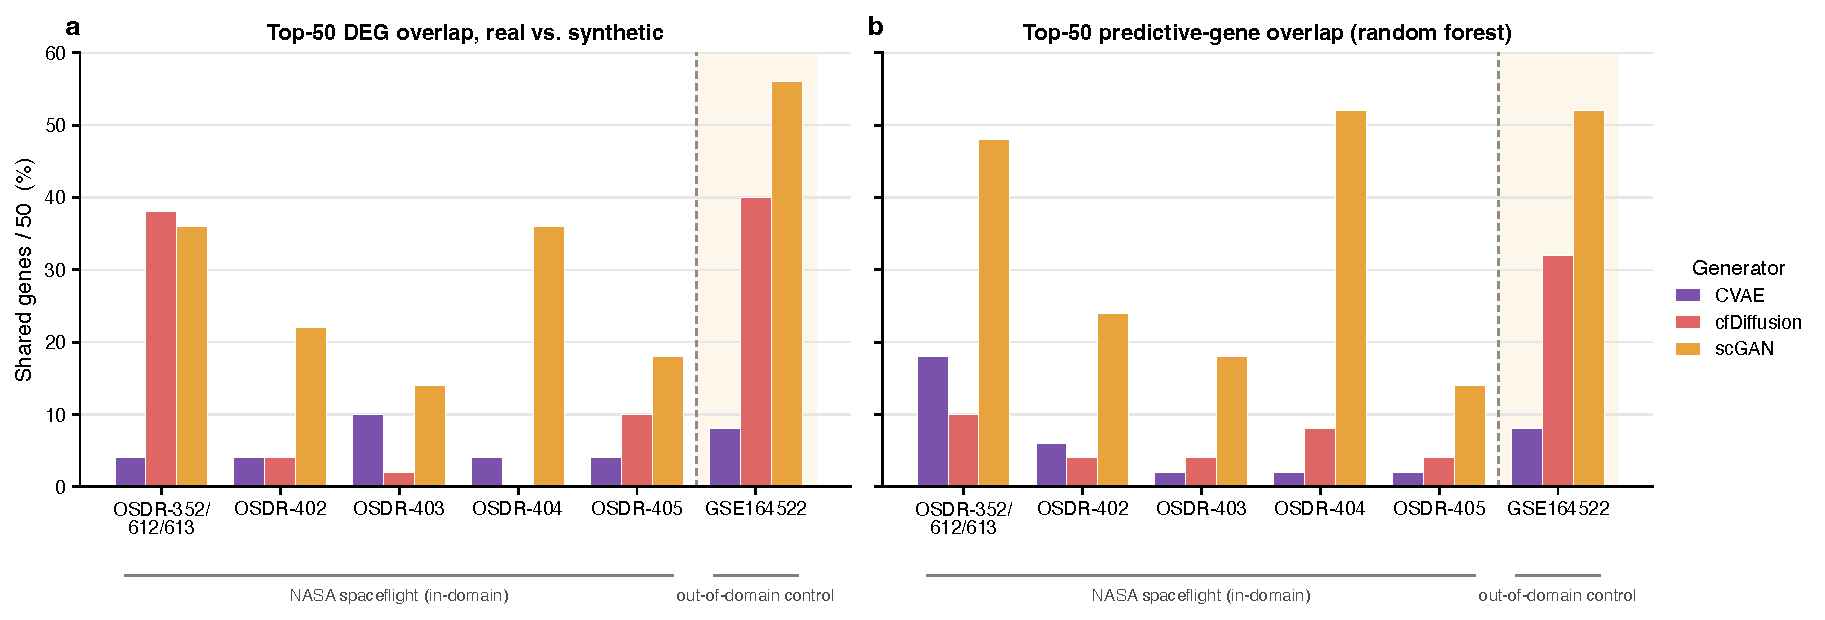
\includegraphics[width=\linewidth]{fig_overlap.pdf}
\caption{\textbf{Condition and phenotype fidelity across datasets.} Top-50 differentially expressed gene overlap (a) and random-forest feature-importance (predictive-gene) overlap (b) between real and synthetic data, grouped by dataset and generator; the shaded column and bracket labels mark the out-of-domain cancer control against the in-domain spaceflight datasets. The multi-conditional scGAN leads on condition fidelity for five of six datasets and on phenotypic fidelity for all six, with the largest margins on the pooled brain set and the two largest-$n$ datasets.}
\label{fig:overlap}
\end{figure}

\begin{figure}[t]
\centering
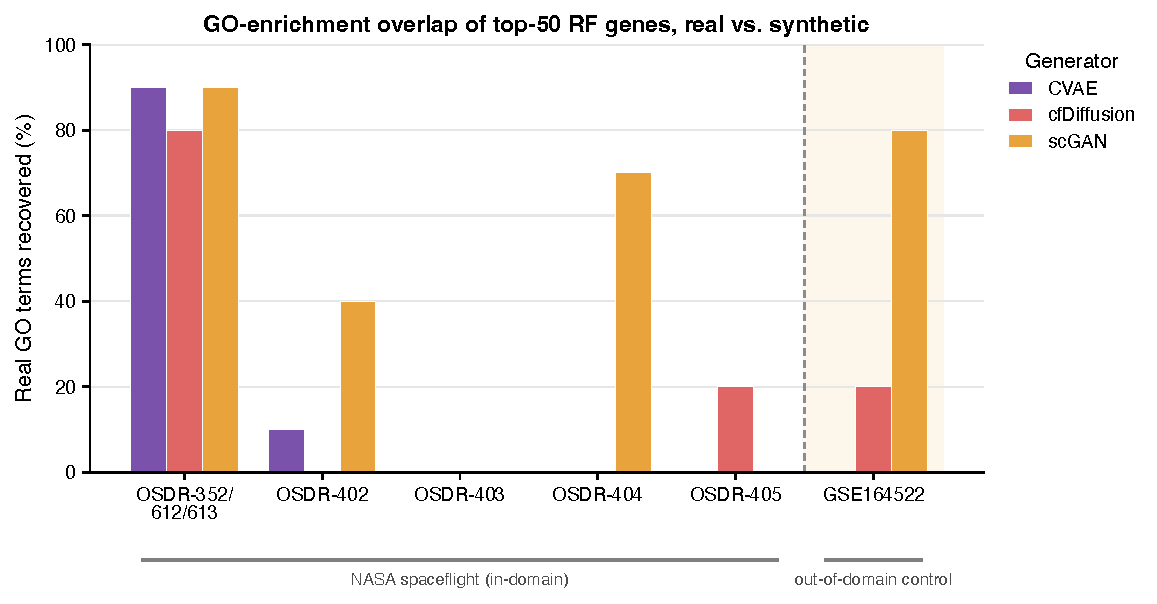
\includegraphics[width=0.82\linewidth]{fig_fgsea.pdf}
\caption{\textbf{Mechanistic fidelity: GO-enrichment overlap of the predictive genes.} Gene-ontology terms over-represented among each model's top-50 random-forest genes (hypergeometric test against MSigDB, top 10 per dataset, FDR $q<0.05$), reported as the percentage of the real data's enriched terms recovered in the synthetic data. Where recoverable signal exists, pathway overlap exceeds gene-level overlap (compare Fig.~\ref{fig:overlap}a): all three generators recover 80 to 90\% of pathways on the pooled brain set, and scGAN recovers 70\% on OSDR-404 and 80\% on the cancer control. Recovered programs are dominated by cytoplasmic translation and ribosomal pathways in spaceflight data and by lymphocyte and T-cell activation in the cancer control; OSDR-403 (bone marrow) shows the opposite case, where tissue-appropriate real enrichment is not recovered by any generator.}
\label{fig:fgsea}
\end{figure}

\begin{figure}[t]
\centering
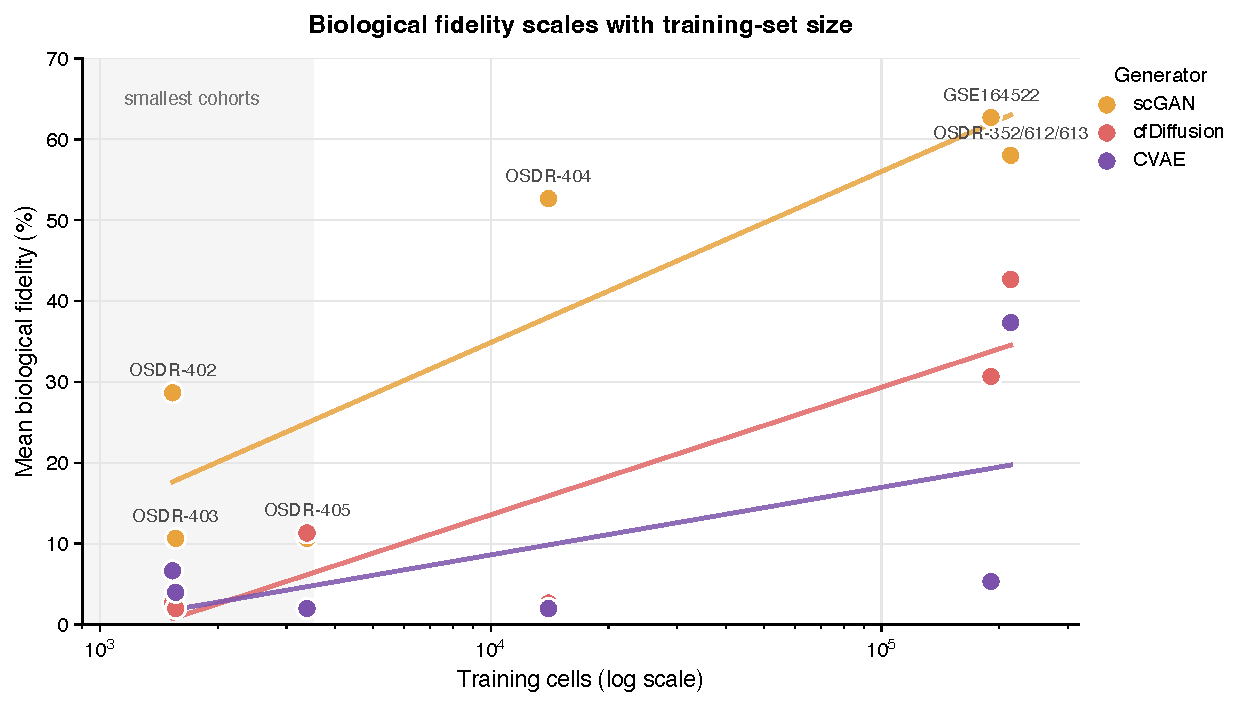
\includegraphics[width=0.78\linewidth]{fig_size_trend.pdf}
\caption{\textbf{Biological fidelity scales with training-set size.} Mean of the three biological-fidelity metrics (top-50 DEG overlap, GO-enrichment overlap, and predictive-gene overlap) per generator against the number of training cells (log scale); lines are least-squares fits in log-cell space. All generators improve with size and the two deep generators scale most steeply; the shaded band marks the smallest cohorts (under 3{,}500 cells).}
\label{fig:size}
\end{figure}

% =====================================================================
\section{Discussion}

\subsection{Biological metrics separate what distributional metrics cannot}
Under a purely distributional lens the generators reach a defined, comparable operating point, yet the \protname{} separates them by asking whether the synthetic data preserves the experimental contrast, the underlying pathways, and the predictive gene programs. The clearest illustration is the CVAE, which attained the highest TSTR accuracy on several datasets while sharing almost none of its important genes with the real classifier: statistical and surface-predictive similarity is necessary but not sufficient, and an evaluation that stops at those numbers can certify synthetic data that has quietly lost the biology it was meant to reproduce. Across these axes the multi-conditional scGAN tended to lead, which we report as a scoping observation on small-sample, multi-conditional data rather than a general ranking, since recent evidence on synthetic scRNA-seq is genuinely mixed \cite{scdiffusion,cfgen,scgft}.

\subsection{Why each layer is necessary}
The layers are ordered to catch distinct failure modes. A model can match the marginal distribution yet scramble the condition contrast; it can preserve the contrast yet miss the pathways that give the contrast meaning; and it can pass all of these yet fail to encode the gene programs that make the data predictive. Gene-level overlap and pathway-level overlap diverged in our data, with pathway overlap higher wherever recoverable signal existed, which is precisely the mechanistic-but-not-mechanical fidelity that matters for discovery. A benchmark that reports only one of these numbers would misrepresent the usefulness of the synthetic data.

\subsection{The sparsity gap constrains the latent-space generators}
The two latent-space generators under-represented dropout severely, with cfDiffusion densest on most datasets, because generating in a compressed latent space discards fine-grained zero structure; the multi-conditional scGAN, which normalizes library size directly in gene space, instead reproduced near-real sparsity. The practical consequence is that the CVAE and cfDiffusion outputs are presently suited to bulk-like and pathway-level analyses rather than to tasks that depend on accurate dropout, such as cell-type identification and trajectory inference, whereas scGAN's output is closer to usable at single-cell resolution. Sparsity-aware objectives, dropout-preserving latent variables analogous to library-size modeling in scVI \cite{scvi}, or count-based likelihoods are natural next steps for the latent-space models.

\subsection{Limitations}
Several limitations bound our claims. The ``first peer-reviewed'' framing is scoped deliberately: generative modeling of spaceflight transcriptomes has previously been demonstrated in bulk RNA-seq, notably with GANs \cite{ganbio}, and a conference-only poster from our group applied a CVAE to spaceflight single-nucleus RNA-seq \cite{ntrs,glare}, so we claim the first peer-reviewed application of GAN and diffusion generative models to spaceflight single-cell data, with a multi-conditional, multi-architecture, biology-aware benchmark, rather than the first generative modeling in the domain. The dataset panel, while at or above the size used by comparable methods papers \cite{cfgen,scdiffusion,cfdiffusion}, remains modest and the individual RRRM-2 studies are small, so we report the spread of metrics across datasets rather than single point estimates, and two low-signal studies (OSDR-403, OSDR-405) recovered little pathway overlap for any model, consistent with the strong dependence of fidelity on cell count (Fig.~\ref{fig:size}). The complementary per-gene distance metrics and formal significance testing were not computed in this run and are left for future work; we lead with feature-importance overlap rather than TSTR accuracy because the latter dissociates from gene-level fidelity. Finally, predictive-gene GO-enrichment overlap is a new synthetic-data metric and would benefit from further validation against held-out biological-signal recovery. We view establishing this methodological foundation as timely, given that larger spaceflight single-cell datasets are only now becoming available.

\subsection{Implications for spaceflight medicine}
Condition-controllable synthetic cells enable in silico cohorts that are impossible to collect from astronauts, supporting power analyses, countermeasure screening across genetic backgrounds, and the development of predictive health models under the sample scarcity that defines this field \cite{scott,ilangovan}. The \protname{} gives the community a way to decide which synthetic data is trustworthy enough for these purposes, and the MMD-stopping rule gives a fair basis for choosing among generators as new architectures arrive.

% =====================================================================
\section{Methods}

\subsection{Datasets and preprocessing}
Spaceflight scRNA-seq datasets were obtained from NASA OSDR and evaluated as five configurations: the individual Rodent Research Reference Mission-2 (RRRM-2) studies OSDR-402 (femur bone marrow), OSDR-403 (humerus bone marrow), OSDR-404 (peripheral blood mononuclear cells), and OSDR-405 (spleen), all from female C57BL/6NTac mice, together with one pooled brain cohort combining OSDR-352, OSDR-612, and OSDR-613 across three strains (Table~\ref{tab:data}). One out-of-domain control, the human colorectal-cancer liver-metastasis tumor-immune atlas GSE164522, was processed identically as a robustness check. Count matrices were library-size normalized to $10^4$ and log$(x+1)$ transformed. Genes expressed in a vanishingly small fraction of cells were removed at a 0.997 sparsity threshold ($3\sigma$ cutoff), and the top 2000 highly variable genes were selected \cite{seurat}. Each dataset was split into training, validation, and held-out test partitions stratified by the primary condition; biological-fidelity metrics were computed on held-out test data to avoid optimistic assessment. The primary condition contrast was spaceflight versus ground control for the OSDR datasets and metastatic-site tumor versus adjacent normal tissue for the cancer control.

\subsection{Shared conditioning vector}
All three generators conditioned on an identical covariate vector, so that the biological comparison reflects the generated data and not differences in conditioning power. For the spaceflight datasets this vector comprised experimental condition (flight versus ground control), biological strain, sex, age at launch, and mission duration; for the cancer control it comprised the major cell-type annotation and tissue compartment. Categorical variables were one-hot encoded and continuous variables were normalized to $[-1,1]$, and the same encoded vector was supplied to every model. This symmetry removes conditioning power as a confounder across the testbed. Because the original cfDiffusion and scGAN implementations condition on a single attribute, we extended both to accept this full multi-attribute vector (below).

\subsection{Conditional variational autoencoder}
The CVAE maps 2000-gene expression vectors to a 32-dimensional latent space through fully connected layers of width $800$ and $400$ with batch normalization, dropout ($0.03$), and nonlinear activations, with the conditioning vector concatenated to the input and again to the latent code before decoding. It maximizes the conditional evidence lower bound,
\begin{equation}
\mathcal{L}_{\mathrm{CVAE}} = \mathbb{E}_{q_\phi(z\mid x,c)}\left[\log p_\theta(x\mid z,c)\right] - \beta\, D_{\mathrm{KL}}\!\left(q_\phi(z\mid x,c)\,\|\,p(z)\right),
\end{equation}
with a Gaussian posterior $q_\phi(z\mid x,c)=\mathcal{N}(z;\mu_\phi(x,c),\sigma_\phi^2(x,c))$, the reparameterization trick for differentiable sampling, a reconstruction term appropriate for normalized expression, and $\beta=0.05$ controlling the Kullback-Leibler regularization. Trained with Adam (learning rate $10^{-2}$, weight decay $10^{-3}$, batch size $128$) in PyTorch.

\subsection{Classifier-free latent diffusion (cfDiffusion)}
Following cfDiffusion \cite{cfdiffusion}, a first-stage variational autoencoder compresses the 2000-gene vectors to a 128-dimensional latent space (encoder $1024\to1024\to128$, decoder reversed; $\beta=10^{-3}$), and a second-stage denoising diffusion model operates in that latent space using a skip-connected network with hidden widths $512,512,256,128$. The forward process adds Gaussian noise over $T=1000$ steps with a cosine schedule $\{\beta_t\}$, $q(z_t\mid z_{t-1})=\mathcal{N}(z_t;\sqrt{1-\beta_t}\,z_{t-1},\beta_t I)$, and the network $\epsilon_\theta(z_t,t,c)$ learns to predict the added noise by minimizing
\begin{equation}
\mathcal{L}_{\mathrm{diff}} = \mathbb{E}_{z_0,c,t,\epsilon}\left[\left\|\epsilon - \epsilon_\theta\!\left(\sqrt{\bar\alpha_t}\,z_0 + \sqrt{1-\bar\alpha_t}\,\epsilon,\; t,\; c\right)\right\|^2\right].
\end{equation}
Classifier-free guidance is enabled by dropping the condition with probability $p_{\mathrm{drop}}=0.1$ during training and combining conditional and unconditional predictions at inference with guidance strength $\gamma=2.0$, $\tilde\epsilon_\theta = \epsilon_\theta(z_t,t,\varnothing) + \gamma\left(\epsilon_\theta(z_t,t,c)-\epsilon_\theta(z_t,t,\varnothing)\right)$. We extended the original single-attribute conditioning to the full multi-attribute vector with a per-attribute embedder bank: each categorical attribute is one-hot encoded and linearly projected, each continuous attribute is linearly projected, each to $128/K$ dimensions for $K$ conditioning attributes; the per-attribute embeddings are concatenated and passed through a linear layer, a nonlinearity, and layer normalization to a single 128-dimensional joint condition embedding. This embedding is injected additively into every residual block alongside the timestep embedding, and under classifier-free dropout (or when an attribute is absent) the corresponding embedding is set to zero, so dropped attributes contribute nothing. Implemented in PyTorch.

\subsection{Multi-conditional scGAN}
The GAN arm is the scGAN architecture of Marouf et al.\ \cite{scgan}, a Wasserstein GAN with gradient penalty and a library-size normalization layer, implemented in TensorFlow. The generator maps a 128-dimensional noise vector through hidden widths $256,512,1024$ to 2000 genes, and the critic mirrors this. The original conditional variant (cscGAN) conditions on a single categorical variable (cell type). We extended it to accept the full multi-attribute conditioning vector used by the other two generators by injecting the covariates through \emph{conditional (feature-wise) batch normalization}: the concatenated condition vector (one-hot categorical plus $[-1,1]$-normalized continuous attributes) is mapped by a small multilayer perceptron to per-layer scale and offset parameters $(\gamma,\beta)$ that modulate each hidden layer's batch-normalized activations in both the generator and the critic, so that generation is controllable on condition, strain, sex, age, and duration jointly. This adaptation simply lets scGAN accept the same conditioning vector as the CVAE and cfDiffusion; it is a means to a fair comparison rather than a modeling contribution in itself. Trained with Adam ($\beta_1=0$, $\beta_2=0.9$, learning rate $1.5\times10^{-4}$ for both generator and critic), gradient-penalty weight $\lambda_{\mathrm{gp}}=15$, four critic updates per generator update, gradient-norm clipping at $1.0$, and batch size $32$.

\subsection{MMD-based, architecture-agnostic stopping rule}
Because ELBO, adversarial, and denoising losses are not comparable across families, we stopped all models on a shared external criterion. We fit a 50-component principal-component analysis once on the real training data only and froze it. The same frozen transform was applied to both real validation data and synthetic data; MMD was never computed in the raw high-dimensional space, where distance concentration renders the radial-basis-function kernel insensitive, nor was the PCA ever refit on synthetic or pooled data. Every five epochs during training, the model generated a synthetic replicate of the validation set, both real and synthetic validation sets were projected through the frozen PCA, and MMD was computed between them with an RBF kernel \cite{gretton,sutherland}. The kernel bandwidth $\sigma$ was set by the median heuristic on the training data using proportional stratified sampling (up to $10^4$ cells). Training continued while MMD improved and stopped when it failed to improve by more than $10^{-3}$ over four consecutive evaluations, giving each generator its own converged operating point. This use of MMD as a shared stopping criterion, so that generators of different families reach a common quality point rather than being halted on incommensurable losses, is a deliberate choice that makes the biological comparison fair: MMD has been used as an evaluation metric \cite{gretton,sutherland} and as a within-family early-stopping signal, but here it serves as the common operating point at which otherwise incomparable generators are evaluated. MMD convergence is treated as a fair common operating point, not as proof that biology has been fully learned.

\subsection{Biological-fidelity protocol}
For every dataset and architecture we generated a full one-to-one replicate of the real dataset, matching the exact distribution of mission parameters (the same combinations of condition, strain, sex, age, and duration), and computed three metrics on held-out test data.

\noindent\textbf{Condition fidelity (DEG overlap).} Differential expression between the two primary groups was computed by t-test separately in real and synthetic data, genes were ranked by absolute log fold change, and the overlap of the top 50 genes was quantified. The value $N=50$ is a convention; the metric is defined for any $N$, and its sensitivity to $N$ is reported in \res{Supplementary Fig.\ SX}.

\noindent\textbf{Mechanistic fidelity (GO-enrichment overlap of the predictive genes).} The top 50 random-forest important genes (the same lists used for phenotypic fidelity, below) were tested for gene-ontology over-representation with \texttt{gseapy} \cite{gseapy} using a hypergeometric test against the MSigDB ontology collections \cite{msigdb} (the full M5 set for mouse, comprising GO:BP, GO:CC, GO:MF and the Mammalian Phenotype Ontology, with gene universe $N=46{,}339$; and the equivalent C5 set for human, $N=43{,}841$), keeping terms at FDR $q<0.05$ and retaining the top ten by $q$-value. Mechanistic fidelity is the directional percentage of the real data's top enriched terms that the synthetic data also recovers. Because the gene set is the classifier's own predictive genes, this captures functional coherence that gene-level overlap can miss while tying the mechanistic test directly to the phenotypic one.

\noindent\textbf{Phenotypic fidelity (RF feature-importance overlap, TSTR).} Random-forest classifiers (100 trees, maximum depth 10, five-fold cross-validation repeated three times, i.e.\ 15 fits) were trained to distinguish the two primary groups, one on synthetic data and one on real data, using the 2000 highly variable genes as features. Genes were ranked by mean Gini importance across the 15 fits, and the top 50 were compared by overlap; these same 50 genes seed the mechanistic layer above. Training on synthetic data and testing on real held-out data (train-on-synthetic, test-on-real \cite{esteban}) inverts the classifier two-sample test of prior work \cite{scgan,scdiffusion,lopezpaz}, in which chance-level discrimination is optimal: here, high agreement is optimal. Because absolute TSTR accuracy dissociated from gene overlap (notably for the CVAE), we report feature-importance overlap as the primary phenotypic-fidelity quantity and accuracy as a secondary measure.

\subsection{Statistical-fidelity distances}
MMD at convergence (frozen PCA-50) is the primary statistical-fidelity quantity. Complementary per-gene distances (cosine, Sinkhorn-approximated Wasserstein, mean absolute deviation of per-gene means, and pooled-covariance Mahalanobis distance) and formal significance testing were not computed in the reported pipeline run and are left for future work.

\subsection{Training and hardware}
All models used Adam optimization with the MMD stopping rule above (learning rate $10^{-2}$ for the CVAE, $10^{-3}$ for the cfDiffusion first-stage VAE, and $1.5\times10^{-4}$ for scGAN). Classifier-free guidance used strength $\gamma=2.0$ with condition-drop probability $0.1$; the gradient-penalty weight was $15$ with four critic updates per generator update. Converged operating points occurred at different epochs per model and dataset (Fig.~\ref{fig:mmd}; Table~\ref{tab:stat}). For evaluation, each model generated a one-to-one synthetic replicate of the corresponding real dataset; diffusion sampling used DDIM with \res{number} steps.

\subsection{Code and data availability}
All scRNA-seq datasets are available in the NASA OSDR \cite{osdr} and, for the cancer control, in GEO under accession GSE164522. Training scripts, trained models, generated data, and the \protname{} implementation are available at \res{repository URL}.

% =====================================================================
\section*{Acknowledgements}
We thank the Space Life Sciences Training Program and the AI4LS team at NASA Ames Research Center for support. \res{Add grant numbers, VIP program acknowledgement, and any additional personnel.}

\section*{Author contributions}
\res{Specify, e.g.: A.S.\ conceived the study, implemented the models and the biological-fidelity protocol, ran experiments, and wrote the manuscript; W.A.\ and J.C.\ supervised and edited.}

\section*{Competing interests}
The authors declare no competing interests.

% =====================================================================
\begin{thebibliography}{99}
\small
\bibitem{twins} Garrett-Bakelman FE, et al. The NASA Twins Study: a multidimensional analysis of a year-long human spaceflight. \textit{Science} 364, eaau8650 (2019). doi:10.1126/science.aau8650.
\bibitem{i4} Overbey EG, et al. Spatial and single-cell profiling of the multiomic response to spaceflight. \textit{Nat.\ Commun.} 15, 4954 (2024). doi:10.1038/s41467-024-48916-8.
\bibitem{ilangovan} Ilangovan V, et al. Machine learning classification of spaceflown versus ground-control mice from harmonized liver transcriptomes. \textit{npj Microgravity} 10, 61 (2024). doi:10.1038/s41526-024-00379-3.
\bibitem{scott} Scott RT, Sanders LM, Antonsen EL, et al. Biomonitoring and precision health in deep space supported by artificial intelligence. \textit{Nat.\ Mach.\ Intell.} 5, 196--207 (2023). doi:10.1038/s42256-023-00618-4.
\bibitem{osdr} Gebre SG, et al. NASA Open Science Data Repository: open science for life in space. \textit{Nucleic Acids Res.} 53, D1697--D1710 (2024). doi:10.1093/nar/gkae1116.
\bibitem{scvi} Lopez R, Regier J, Cole MB, Jordan MI, Yosef N. Deep generative modeling for single-cell transcriptomics. \textit{Nat.\ Methods} 15, 1053--1058 (2018). doi:10.1038/s41592-018-0229-2.
\bibitem{activa} Heydari AA, Davalos OA, Zhao L, Hoyer KK, Sindi SS. ACTIVA: realistic single-cell RNA-seq generation with automatic cell-type identification using introspective variational autoencoders. \textit{Bioinformatics} 38, 2194--2201 (2022). doi:10.1093/bioinformatics/btac095.
\bibitem{scgan} Marouf M, et al. Realistic in silico generation and augmentation of single-cell RNA-seq data using generative adversarial networks. \textit{Nat.\ Commun.} 11, 166 (2020). doi:10.1038/s41467-019-14018-z.
\bibitem{scdiffusion} Luo E, Hao M, Wei L, Zhang X. scDiffusion: conditional generation of high-quality single-cell data using diffusion model. \textit{Bioinformatics} 40, btae518 (2024). doi:10.1093/bioinformatics/btae518.
\bibitem{cfdiffusion} Zhang T, Zhao Z, Ren J, Zhang Z, Zhang H, Wang G. cfDiffusion: diffusion-based efficient generation of high-quality scRNA-seq data with classifier-free guidance. \textit{Brief.\ Bioinform.} 26, bbaf071 (2025). doi:10.1093/bib/bbaf071.
\bibitem{cfgen} Palma A, et al. Multi-modal and multi-attribute generation of single cells with CFGen. \textit{Proc.\ ICLR} (2025). arXiv:2407.11734.
\bibitem{scgft} Tedesco M, et al. Single-cell generative modeling with the Fourier transform (scGFT). \textit{Commun.\ Biol.} 8, 1 (2025). doi:10.1038/s42003-025-07552-8.
\bibitem{scdesign3} Song D, et al. scDesign3 generates realistic in silico data for multimodal single-cell and spatial omics. \textit{Nat.\ Biotechnol.} 41, 1610--1618 (2023). doi:10.1038/s41587-023-01772-1.
\bibitem{simbench} Cao Y, Yang P, Yang JYH. A benchmark study of simulation methods for single-cell RNA sequencing data. \textit{Nat.\ Commun.} 12, 6911 (2021). doi:10.1038/s41467-021-27130-w.
\bibitem{gretton} Gretton A, Borgwardt KM, Rasch MJ, Sch\"olkopf B, Smola A. A kernel two-sample test. \textit{J.\ Mach.\ Learn.\ Res.} 13, 723--773 (2012).
\bibitem{sutherland} Sutherland DJ, et al. Generative models and model criticism via optimized maximum mean discrepancy. \textit{Proc.\ ICLR} (2017). arXiv:1611.04488.
\bibitem{gseapy} Fang Z, Liu X, Peltz G. GSEApy: a comprehensive package for performing gene set enrichment analysis in Python. \textit{Bioinformatics} 39, btac757 (2023). doi:10.1093/bioinformatics/btac757.
\bibitem{msigdb} Liberzon A, Birger C, Thorvaldsd\'ottir H, Ghandi M, Mesirov JP, Tamayo P. The Molecular Signatures Database (MSigDB) hallmark gene set collection. \textit{Cell Syst.} 1, 417--425 (2015). doi:10.1016/j.cels.2015.12.004.
\bibitem{esteban} Esteban C, Hyland SL, R\"atsch G. Real-valued (medical) time series generation with recurrent conditional GANs. \textit{arXiv} 1706.02633 (2017).
\bibitem{lopezpaz} Lopez-Paz D, Oquab M. Revisiting classifier two-sample tests. \textit{Proc.\ ICLR} (2017). arXiv:1610.06545.
\bibitem{seurat} Hafemeister C, Satija R. Normalization and variance stabilization of single-cell RNA-seq data using regularized negative binomial regression. \textit{Genome Biol.} 20, 296 (2019). doi:10.1186/s13059-019-1874-1.
\bibitem{tenx} Zheng GXY, et al. Massively parallel digital transcriptional profiling of single cells. \textit{Nat.\ Commun.} 8, 14049 (2017). doi:10.1038/ncomms14049.
\bibitem{ntrs} Golts A, Casaletto J, Costes SV. \res{Conditional variational autoencoder for spaceflight single-nucleus RNA-seq (poster title to confirm).} NASA Technical Reports Server (NTRS) (2024).
\bibitem{glare} \res{Authors to confirm.} GLARE: augmentation framework for spaceflight omics. \textit{npj Microgravity} (2025). doi:10.1038/s41526-025-00525-5.
\bibitem{ganbio} \res{Authors to confirm.} Generative adversarial networks for biomarker discovery from NASA OSDR transcriptomes. \textit{Neuroinformatics} (2025). doi:10.1007/s12021-025-09729-2.
\end{thebibliography}

\end{document}
